\documentclass[pdftex,12pt,a4paper]{article}
\pdfpagewidth 8.5in
\pdfpageheight 11.6in
\linespread{1.3}
\usepackage{anysize}
\marginsize{2.5cm}{2.5cm}{2.5cm}{2.5cm}

\usepackage[utf8]{inputenc}
\usepackage[T1]{fontenc}
\usepackage[english]{babel}
\usepackage{indentfirst}
\usepackage{amsmath}
\usepackage{float}
\usepackage{graphicx}
\usepackage{braket}
\usepackage[unicode,pdftex]{hyperref}
%\usepackage{hyperref}
\usepackage{breqn}

\usepackage{listings}
\usepackage{xcolor}

\definecolor{codegreen}{rgb}{0,0.6,0}
\definecolor{codegray}{rgb}{0.3,0.3,0.3}
\definecolor{codepurple}{rgb}{0.58,0,0.82}
\definecolor{backcolour}{rgb}{0.90,0.90,0.87}

\lstdefinestyle{mystyle}{
    backgroundcolor=\color{backcolour},   
    commentstyle=\color{codegreen},
    keywordstyle=\color{magenta},
    numberstyle=\small\color{codegray},
    stringstyle=\color{codepurple},
    basicstyle=\ttfamily\small,
    breakatwhitespace=false,         
    breaklines=true,                 
    captionpos=b,                    
    keepspaces=true,                 
    numbers=left,                    
    numbersep=5pt,                  
    showspaces=false,                
    showstringspaces=false,
    showtabs=false,                  
    tabsize=2
}
\lstset{style=mystyle}

\DeclareMathOperator{\Ai}{Ai}
\DeclareMathOperator{\Bi}{Bi}
\DeclareMathOperator{\Aip}{Ai^\prime}
\DeclareMathOperator{\Bip}{Bi^\prime}
\DeclareMathOperator{\Ti}{Ti}
\DeclareMathOperator{\ctg}{ctg}
\DeclareMathOperator{\sgn}{sgn}
%\DeclareMathOperator{\max}{max}
\let\Im\relax
\DeclareMathOperator{\Im}{Im}
\DeclareMathOperator{\Tr}{Tr}
\newcommand{\op}[1]{\hat{#1}}
\newcommand{\norm}[1]{\left\lVert #1 \right\rVert}
\newcommand*\Laplace{\mathop{}\!\mathbin\bigtriangleup}

\newcommand{\aeqref}[1]{\az{\eqref{#1}}}
\newcommand{\Aeqref}[1]{\Az{\eqref{#1}}}

\hypersetup{
    colorlinks,
    citecolor=black,
    filecolor=black,
    linkcolor=black,
    urlcolor=black
}
\hypersetup{	
	pdftitle={Gamma spectroscopy},
	pdfauthor={Kürti Zoltán}}

\frenchspacing
\begin{document}

	\centerline{\bf\LARGE Gamma spectroscopy}

	\vskip0.4truein\centerline{\Large\sc Kürti Zoltán}\vskip0.10truein
	%\centerline{\includegraphics[scale=0.5]{./elte_cimer_color.pdf}}
	\vskip0.4truein
	\centerline{\Large Group B}\vskip0.2truein
	\centerline{\Large{Measurement date: November 4, 2021.}}\vskip0.2truein
	\centerline{\Large{Hand in date: \today}}\vskip0.2truein
	\thispagestyle{empty}
	\newpage
	\tableofcontents
	\newpage
	\section{Introduction}
		The goal of this laboratory class was to to measure the gamma radiation emitted by radioactive isotopes. Alpha and beta decays release energy on the order of one up to a couple MeV. Alpha decays are strong processes, meaning they can be described by diagrams involving pion exchanges (at a deeper level this is a result of gluon exchanges, the strong interaction). Beta decays is a result of the weak interaction causing a flavor change ($u \rightarrow d$ in the case of negative beta decay) mediated by the $W^{\pm}$ bosons. Some of the available energy is carried away by the electrons and neutrinos in beta decays, alpha particles in alpha decays. This process leaves an excited nucleus behind. Gamma photons are emitted as these excited nuclei reach their ground states. Based on the measured spectra both the isotope type and the activity of the isotope can be determined.
	\subsection{Measurement setup}
		The two main parts of the measurement setup were the HPGe detector and the amplitude analyzer. HPGe stands for high purity germanium, this makes up the sensitive part of the detector. The rest of the detector consists of protective casing and electronics. Incoming ionizing radiation creates electron-hole pairs. The number of created pairs is to good approximation proportional to the energy absorbed by the semiconductor. The detector is indirectly connected to a liquid nitrogen bath, which cools down the detector considerably. This makes it that thermal fluctuations don't create a significant number of electron-hole pairs, so the only source of current that is measured comes from electron-hole pairs created by the ionizing radiation. These pairs are prohibited from recombining by the high voltage connected to the germanium detector.
		
		The other key component is the amplitude analyzer. It measures the charge carried by electric impulses. This charge is directly proportional to the number of electron-hole pairs created during the time interval of the pulse and therefore characteristic of the energy of the incoming radiation. Based on this charge the amplitude analyzer chooses the corresponding energy bin, and increments the counter corresponding to that bin by one. Finally this analyzer is connected to a computer, where the data is interpreted and displayed. The relation between the bin numbers and the energy of the radiation is expected to be linear, but the exact parameters of the relation are not known before calibration.
	\section{Calibration}
		To determine the parameters of the linear relation between bin number and energy, peaks with known energy are needed to be measured. The linear relationship is expected based on reasoning described in the previous paragraph. During our measurement we used $^{232}\text{Th}$ isotope. The energy of two easily identifiable gamma peaks is known The first one is $238.6\text{keV}$, this is the peak with the largest intensity. The other characteristic peak is at $2614.7keV$, this is the highest energy peak observed. These peaks were identified in the spectrum. To validate the identification of peaks, after using the two peaks to calibrate the linear relation between energy and bin number, other peaks of the $^{232}\text{Th}$ isotope were identified and we checked if their energy matches up with the values read off from tables. These other peaks were at $580keV$ and $908keV$ according to the calibration. These are the $583.191keV$ and $911.316keV$ peaks respectively, both corresponding to $^{208}\text{Tl}$, which is part of the thorium series. The linear fit for energy was
		\begin{equation}
			E = 1.3247keV \cdot n - 4.6keV,
		\end{equation}
		where $n$ is the bin number. From the validation we know the energy measured from the bin number is accurate within a couple $keV$. This is precise enough to identify peaks. The source of the error is that the current impulse coming fro the HPGe detector isn't exactly in linear relation with the energy absorbed by the detector.
	\section{Granite sample}
		The first sample we examined after calibration was a granite rock sample. Table \ref{granitedata}. contains the data required for the activity calculations.
		\begin{table}[H]
		\centering
		\begin{tabular}{|c|c|c|c|c|c|c|}
			\hline
			Energy [$keV$] & Net area & Net area   & Intensity & $\eta$ & $\eta$ rel. & Isotope \\
			               &          & rel. error &           &        & error       &         \\
			\hline
            $351.3$ & $36043$ & $0.6\%$ & 3.689e-01 & $2.198\%$ & $9.0\%$ & $^{214}\text{Pb}$ \\
            $999.1$ & $620$ & $14.2\%$ & 8.320e-03 & $0.846\%$ & $7.6\%$ & $^{234}\text{Pa}$ \\
            $186.7$ & $12230$ & $1.1\%$ & 3.280e-02 & $3.137\%$ & $9.1\%$ & $^{226}\text{Ra}$ \\
            $295.0$ & $23525$ & $0.9\%$ & 1.919e-01 & $2.042\%$ & $6.6\%$ & $^{214}\text{Pb}$ \\
            $1765.1$ & $4430$ & $1.9\%$ & 1.620e-01 & $0.452\%$ & $8.8\%$ & $^{214}\text{Bi}$ \\
            $1118.6$ & $5706$ & $2.0\%$ & 1.550e-01 & $0.702\%$ & $9.3\%$ & $^{214}\text{Bi}$ \\
            $242.1$ & $10554$ & $1.7\%$ & 7.453e-02 & $2.609\%$ & $8.7\%$ & $^{214}\text{Pb}$ \\
			\hline
		\end{tabular}
		\caption{Granite sample data}
		 \label{granitedata}
		\end{table}
		The spectrum was taken over a period of $1000s$. From this the activity can be calculated using
		\begin{equation}
			A = \frac{N}{I\eta t},
			\label{activity}
		\end{equation}
		with error
		\begin{equation}
			\sigma_{\text{rel}}(A) = \sqrt{\sigma_{\text{rel}}(\eta)^2 + \sigma_{\text{rel}}(N)^2}.
		\end{equation}
		These equations give the results in table \ref{granitepeaks}.
		\begin{table}[H]
		\centering
		\begin{tabular}{|c|c|c|c|}
			\hline
			Energy [$keV$] & Activity [$kBq$]& Activity error [$kBq$]& Isotope \\
			\hline
            $351.3$ & $4.4$ & $0.4$ & $^{214}\text{Pb}$ \\
            $999.1$ & $8.8$ & $1.4$ & $^{234}\text{Pa}$ \\
            $186.7$ & $11.9$ & $1.1$ & $^{226}\text{Ra}$ \\
            $295.0$ & $6.0$ & $0.4$ & $^{214}\text{Pb}$ \\
            $1765.1$ & $6.1$ & $0.5$ & $^{214}\text{Bi}$ \\
            $1118.6$ & $5.2$ & $0.5$ & $^{214}\text{Bi}$ \\
            $242.1$ & $5.4$ & $0.5$ & $^{214}\text{Pb}$ \\
			\hline
		\end{tabular}
		\caption{The activities corresponding to peaks in the granite sample.}
		 \label{granitepeaks}
		\end{table}
		Corresponding peaks can be averaged. The correct way to calculate the average given that we know the uncertainties is the following,
		\begin{equation}
			\langle A\rangle = \frac{\sum_i A_i / \sigma_i^2}{\sum_i 1 / \sigma_i^2}.
		\end{equation}
		The uncertainty of this averaged number is
		\begin{equation}
			\sigma_A = \frac{1}{\sqrt{\sum_i 1 / \sigma_i^2}}.
		\end{equation}
		With the above formula I determined the combined activity of the lead and bismuth isotopes. To determine if a significant fraction of the radon gas escapes the granite sample I also calculated the weighted average of the isotope after the radon in the decay chain and compared it to the protactinium peak. I did not use the $186keV$ peak in this calculation because significant area of the $186keV$ peak corresponds to $^{235}\text{U}$. The results are summed up in table \ref{graniteaverages}. and in figure \ref{graniteaveragesfig}.
		\begin{table}[H]
		\centering
		\begin{tabular}{|c|c|c|}
			\hline
			Group & Activity [$Bq$] & Activity error [$Bq$] \\
			\hline
            $^{214}\text{Pb}$ & 5282 & 244 \\
            $^{214}\text{Bi}$ & 5614 & 367 \\
            $^{234}\text{Pa}$ & 8812 & 1421 \\
            After $^{222}\text{Rn}$ & 5384 & 203 \\
            \hline
		\end{tabular}
		\caption{Averaged activities of the granite sample}
		\label{graniteaverages}
		\end{table}
		\begin{figure}[H]
			\centering
			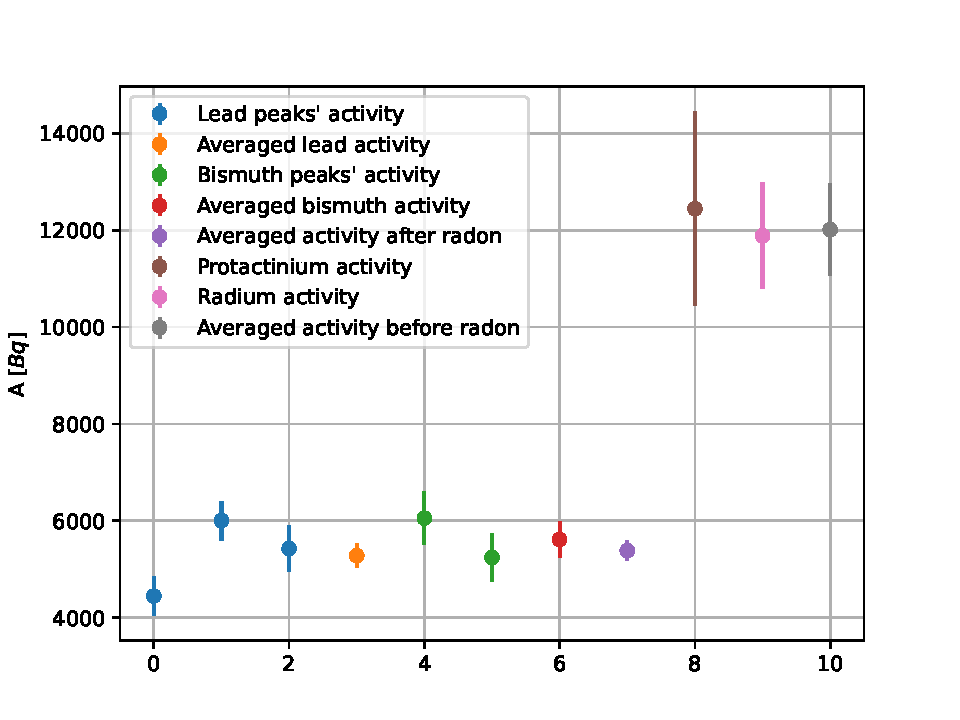
\includegraphics[scale=1]{./figs/graniteactivities.pdf}
			\caption{Graphical representation of activities and errors corresponding to peaks and their averages.}
			\label{graniteaveragesfig}
		\end{figure}
		
		%From figure \ref{graniteaveragesfig}. it can be seen that the error in the activity corresponding to the $186keV$ radium peak and the $1001keV$ protactinium peak is large compared to their difference. This means the amount of $^{235}\text{U}$, which would contribute to the $186keV$ peak can not be determined from this measurement. $0.7 \%$ $^{235}\text{U}$ contributes
		%\begin{equation}
		%	\frac{0.7 \% \lambda_{235}}{0.7 \% \lambda_{235} + 99.3 \% \lambda_{238}} = 4.3 \%
		%\end{equation}
		%to the $186keV$ peak. The relative error in the activity of the $186keV$ peak is $9.2\%$ and $16.1\%$ for the $1001keV$ peak. The intensity corresponding to the $^{235}\text{U}$ is roughly 16 times larger compared to the $186keV$ emission of $^{226}\text{Ra}$. Based on these numbers a rough estimate for the most amount of $^{235}\text{U}$ consistent with the measured data is $\sqrt{9.2\%^2 + 16.1\%^2} / 4.3\% / 16 = 0.27\%$. However this does not account for any systematic errors. One possible error I could think of is that the region of interest selected was too small for the $186keV$ peak. The region of interest was from $184.85keV$ to $188.82$, the FWHM was $2.04keV$ and the centroid $186.69keV$. Based on this data at least some of the error is likely explained by a too small region of interest, as for other peaks the region width and FWHM ratio was higher. Other sources of error could be unaccounted differences in $\mu$, as the the Monte-Carlo simulation did miss some of the details of the setup.
		
		We can estimate the amount of radon gas that escapes the rock sample before decaying.
		\begin{equation}
			r = \frac{A_1 - A_2}{A_1},
		\end{equation}
		where $r$ is the ratio of radon gas that escapes before decaying, $A_1$ and $A_2$ are the averaged activities measured from elements before and after the radon in the decay chain, respectively. The error of this ratio is given by
		\begin{equation}
			\sigma_r = \sigma\left(1 - \frac{A_2}{A_1}\right) = \frac{A_2}{A_1}\sqrt{\left(\frac{\sigma_{A_1}}{A_1}\right)^2 + \left(\frac{\sigma_{A_2}}{A_2}\right)^2}.
		\end{equation}
		The result of this calculation is that $(38.9\pm1.0)\%$ of the radon gas escapes the granite sample before decaying.
		
		From the activity of protactinium, which is before the radon gas, the amount of $^{238}\text{U}$ can be calculated using its decay rate. This is because this isotopes is guaranteed to be in secular equilibrium granted the rock formed sufficiently long ago. The peak corresponding to radium can not be used, because $^{235}\text{U}$ also has a peak at $186keV$.
		\begin{equation}
			N = \frac{A}{\lambda},
		\end{equation}
		\begin{equation}
			\sigma_N = \frac{\sigma_A}{\lambda},
		\end{equation}
		where $\lambda = \frac{\log(2)}{T_{1/2}} = 4.92\cdot 10^{-18}\frac{1}{s}$ is the decay rate of $^{238}\text{U}$. From this the number of $^{238}\text{U}$ atoms in the granite sample is $(1.79\pm0.29)\cdot 10^{21}$, which corresponds to a mass of $(0.71\pm0.11)g$ $^{238}\text{U}$ in the granite sample. Knowing that the mass of the granite sample was $280g$, the $^{238}\text{U}$ concentration of the sample is $(2530\pm410)g/ton$.
		
		The $^{235}\text{U}$ content can be calculated the following way. The activity of protactinium and radium is the same as they are both isotopes before radon in the decay chain. However the $186keV$ peak corresponding to radium gets contribution from the decay chain of $^{235}\text{U}$. Based on the difference the $^{235}\text{U}$ content can be determined. It is important that the difference is taken between the measured and expected net areas. This is because the intensity corresponding to the $186keV$ peak is different for radium and the $^{235}\text{U}$ decay chain. Following this logic, the expected net area corresponding to $^{226}\text{Ra}$ is
		\begin{equation}
			N_{\text{Ra}-226} = N_{\text{Pa}-234}\frac{I_{\text{Ra}-226}\mu_{186keV}}{I_{\text{Pa}-234}{\mu_{1001keV}}}.
		\end{equation}
		$\mu$ are the detector efficiencies at the peak energies, while $I$ are the intensities (probabilities) corresponding to the relevant photons. These $\mu$ and $I$ values are listed in table \ref{granitepeaks}. The difference gives the net area corresponding to the $186keV$ peak of ${235\text{U}}$,
		\begin{equation}
			N_{235} = N_{186keV} - N_{\text{Ra}-226}.
		\end{equation}
		Here $N_{186keV}$ corresponds to the measured net area of the $186keV$ peak, $N_{\text{Ra}-226}$ is calculated with the previous formula. Finally $N_{235}$ is the net area corresponding to $^{235\text{U}}$. Using \eqref{activity} the activity of $^{235\text{U}}$ is
		\begin{equation}
			A_{\text{U}-235} = \frac{N_{235}}{I_{\text{U}-235}\mu_{186keV} t} = \frac{N_{186keV}}{I_{\text{U}-235}\mu_{186keV} t} - \frac{I_{\text{Ra}-226}}{I_{\text{U}-235}}\frac{N_{\text{Pa}-234}}{I_{\text{Pa}-234}\mu_{1001keV} t}.
		\end{equation}
		This gives $^{235}\text{U}$ content of $m_{235} = (0.0023\pm0.0014)g$, which is $(0.33\pm0.2)\%$ with respect to the mass of all uranium in the sample.
	\section{Soil sample}
		The data of the measured peaks from the soil sample are summarized in table \ref{soildata}.
		\begin{table}[H]
		\centering
		\begin{tabular}{|c|c|c|c|c|c|c|}
			\hline
			Energy [$keV$] & Net area & Net area   & Intensity & $\eta$ & $\eta$ rel. & Isotope \\
			               &          & rel. error &           &        & error       &         \\
			\hline
            $658.5$ & $407$ & $5.7\%$ & 8.998e-01 & $1.1082\%$ & $8.6\%$ & $^{134}\text{Cs}$ ($^{134}\text{Ba}$) \\
            $120.9$ & $437$ & $6.6\%$ & 2.843e-01 & $3.3051\%$ & $7.7\%$ & $^{152}\text{Eu}$ \\
            $343.4$ & $172$ & $9.9\%$ & 2.649e-01 & $1.6480\%$ & $8.2\%$ & $^{152}\text{Eu}$ \\
            $1405.3$ & $27$ & $22.8\%$ & 2.075e-01 & $0.4523\%$ & $8.9\%$ & $^{152}\text{Eu}$ \\
            $776.7$ & $50$ & $22.4\%$ & 1.274e-01 & $0.9176\%$ & $8.9\%$ & $^{152}\text{Eu}$ \\
            $244.9$ & $65$ & $14.6\%$ & 7.494e-02 & $2.5473\%$ & $9.5\%$ & $^{152}\text{Eu}$ \\
			\hline
		\end{tabular}
		\caption{Soil sample data. The $658.5keV$ peak is emitted by $^{134}\text{Ba}$ after a $^{134}\text{Cs}$ beta decays.}
		\label{soildata}
		\end{table}
		The first peak is emitted by a transition of the barium atom, after a cesium atom decays into it. The activities can be calculated in the same ways as for the granite sample. The results are listed in table \ref{soilpeaks}.
		\begin{table}[H]
		\centering
		\begin{tabular}{|c|c|c|c|}
			\hline
			Energy [$keV$] & Activity [$kBq$]& Activity error [$kBq$]& Isotope \\
			\hline
            $658.5$ & $44.8$ & $4.6$ & $^{134}\text{Cs}$ ($^{134}\text{Ba}$) \\
            $120.9$ & $51.0$ & $5.2$ & $^{152}\text{Eu}$ \\
            $343.4$ & $43.3$ & $5.5$ & $^{152}\text{Eu}$ \\
            $1405.3$ & $31.6$ & $7.7$ & $^{152}\text{Eu}$ \\
            $776.7$ & $46.9$ & $11.3$ & $^{152}\text{Eu}$ \\
            $244.9$ & $37.4$ & $6.5$ & $^{152}\text{Eu}$ \\
            \hline
		\end{tabular}
		\caption{The activities corresponding to peaks in the soil sample. The $658.5keV$ peak is emitted by $^{134}\text{Ba}$ after a $^{134}\text{Cs}$ beta decays.}
		\label{soilpeaks}
		\end{table}
		Averaging the europium peaks' activities as in the case of the granite sample I got $(43.2\pm 2.9)Bq$. These activities are visually represented by figure \ref{soilaveragesfig}.
			\begin{figure}[H]
			\centering
			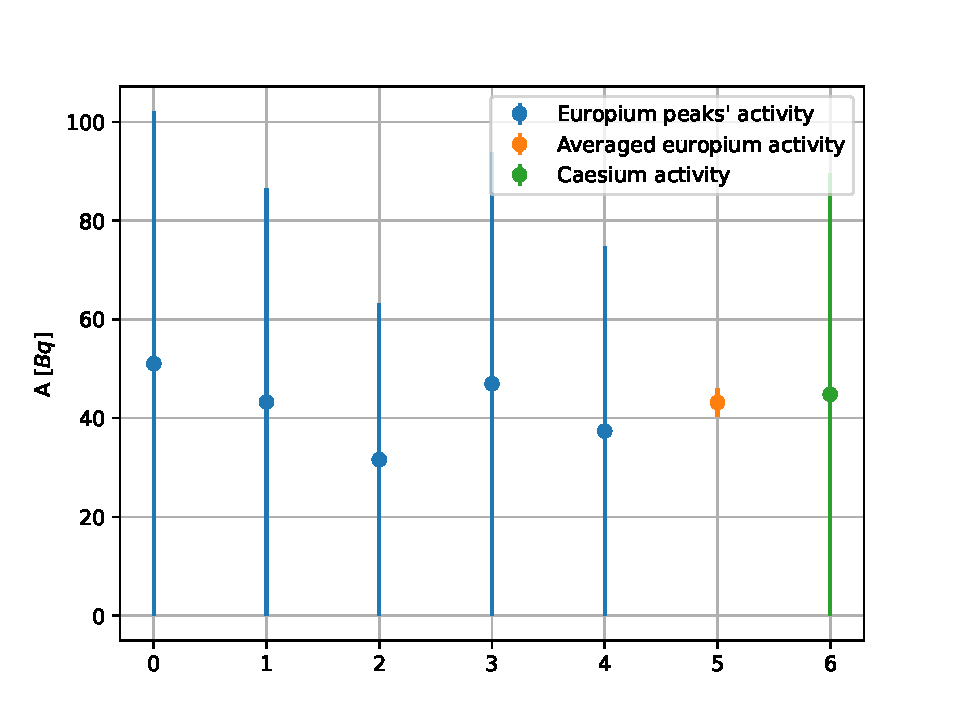
\includegraphics[scale=1]{./figs/soilactivities.pdf}
			\caption{Graphical representation of activities and errors corresponding to peaks and their averages.}
			\label{soilaveragesfig}
		\end{figure}
	\section{Conclusion}
		The lab introduced us to gamma spectroscopy and analyzing the data obtained. In the first part we calibrated the measurement with a thorium sample. The next part was about taking the spectrum of a granite sample and identifying the peaks seen. During evaluation I concluded that a significant portion of the radon gas escapes the sample. The uranium-235 concentration estimated based on the $186keV$ and $1001keV$ peaks is a bit lower than expected. A possible source of this error could be the incorrect selection of the region of interest around the $186keV$ peak. The FWHM to region width ratio was 1.2-2 times as high for the $186keV$ peak as for the other peaks. I also determined the uranium content of the sample. Finally I repeated some of the calculations for a soil sample from near a nuclear bomb test.
	\bibliographystyle{abeld}
    %\bibliography{ref}
\end{document}